\documentclass[1p]{elsarticle_modified}
%\bibliographystyle{elsarticle-num}

%\usepackage[colorlinks]{hyperref}
%\usepackage{abbrmath_seonhwa} %\Abb, \Ascr, \Acal ,\Abf, \Afrak
\usepackage{amsfonts}
\usepackage{amssymb}
\usepackage{amsmath}
\usepackage{amsthm}
\usepackage{scalefnt}
\usepackage{amsbsy}
\usepackage{kotex}
\usepackage{caption}
\usepackage{subfig}
\usepackage{color}
\usepackage{graphicx}
\usepackage{xcolor} %% white, black, red, green, blue, cyan, magenta, yellow
\usepackage{float}
\usepackage{setspace}
\usepackage{hyperref}

\usepackage{tikz}
\usetikzlibrary{arrows}

\usepackage{multirow}
\usepackage{array} % fixed length table
\usepackage{hhline}

%%%%%%%%%%%%%%%%%%%%%
\makeatletter
\renewcommand*\env@matrix[1][\arraystretch]{%
	\edef\arraystretch{#1}%
	\hskip -\arraycolsep
	\let\@ifnextchar\new@ifnextchar
	\array{*\c@MaxMatrixCols c}}
\makeatother %https://tex.stackexchange.com/questions/14071/how-can-i-increase-the-line-spacing-in-a-matrix
%%%%%%%%%%%%%%%

\usepackage[normalem]{ulem}

\newcommand{\msout}[1]{\ifmmode\text{\sout{\ensuremath{#1}}}\else\sout{#1}\fi}
%SOURCE: \msout is \stkout macro in https://tex.stackexchange.com/questions/20609/strikeout-in-math-mode

\newcommand{\cancel}[1]{
	\ifmmode
	{\color{red}\msout{#1}}
	\else
	{\color{red}\sout{#1}}
	\fi
}

\newcommand{\add}[1]{
	{\color{blue}\uwave{#1}}
}

\newcommand{\replace}[2]{
	\ifmmode
	{\color{red}\msout{#1}}{\color{blue}\uwave{#2}}
	\else
	{\color{red}\sout{#1}}{\color{blue}\uwave{#2}}
	\fi
}

\newcommand{\Sol}{\mathcal{S}} %segment
\newcommand{\D}{D} %diagram
\newcommand{\A}{\mathcal{A}} %arc


%%%%%%%%%%%%%%%%%%%%%%%%%%%%%5 test

\def\sl{\operatorname{\textup{SL}}(2,\Cbb)}
\def\psl{\operatorname{\textup{PSL}}(2,\Cbb)}
\def\quan{\mkern 1mu \triangleright \mkern 1mu}

\theoremstyle{definition}
\newtheorem{thm}{Theorem}[section]
\newtheorem{prop}[thm]{Proposition}
\newtheorem{lem}[thm]{Lemma}
\newtheorem{ques}[thm]{Question}
\newtheorem{cor}[thm]{Corollary}
\newtheorem{defn}[thm]{Definition}
\newtheorem{exam}[thm]{Example}
\newtheorem{rmk}[thm]{Remark}
\newtheorem{alg}[thm]{Algorithm}

\newcommand{\I}{\sqrt{-1}}
\begin{document}

%\begin{frontmatter}
%
%\title{Boundary parabolic representations of knots up to 8 crossings}
%
%%% Group authors per affiliation:
%\author{Yunhi Cho} 
%\address{Department of Mathematics, University of Seoul, Seoul, Korea}
%\ead{yhcho@uos.ac.kr}
%
%
%\author{Seonhwa Kim} %\fnref{s_kim}}
%\address{Center for Geometry and Physics, Institute for Basic Science, Pohang, 37673, Korea}
%\ead{ryeona17@ibs.re.kr}
%
%\author{Hyuk Kim}
%\address{Department of Mathematical Sciences, Seoul National University, Seoul 08826, Korea}
%\ead{hyukkim@snu.ac.kr}
%
%\author{Seokbeom Yoon}
%\address{Department of Mathematical Sciences, Seoul National University, Seoul, 08826,  Korea}
%\ead{sbyoon15@snu.ac.kr}
%
%\begin{abstract}
%We find all boundary parabolic representation of knots up to 8 crossings.
%
%\end{abstract}
%\begin{keyword}
%    \MSC[2010] 57M25 
%\end{keyword}
%
%\end{frontmatter}

%\linenumbers
%\tableofcontents
%
\newcommand\colored[1]{\textcolor{white}{\rule[-0.35ex]{0.8em}{1.4ex}}\kern-0.8em\color{red} #1}%
%\newcommand\colored[1]{\textcolor{white}{ #1}\kern-2.17ex	\textcolor{white}{ #1}\kern-1.81ex	\textcolor{white}{ #1}\kern-2.15ex\color{red}#1	}

{\Large $\underline{12n_{0828}~(K12n_{0828})}$}

\setlength{\tabcolsep}{10pt}
\renewcommand{\arraystretch}{1.6}
\vspace{1cm}\begin{tabular}{m{100pt}>{\centering\arraybackslash}m{274pt}}
\multirow{5}{120pt}{
	\centering
	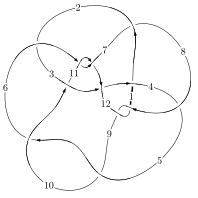
\includegraphics[width=112pt]{../../../GIT/diagram.site/Diagrams/png/2917_12n_0828.png}\\
\ \ \ A knot diagram\footnotemark}&
\allowdisplaybreaks
\textbf{Linearized knot diagam} \\
\cline{2-2}
 &
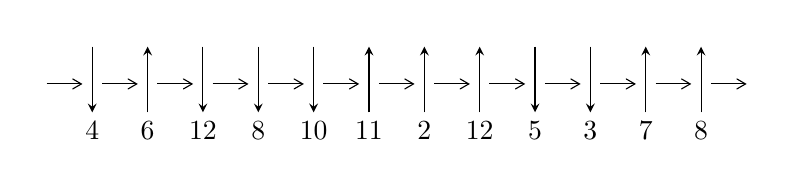
\begin{tikzpicture}[x=20pt, y=17pt]
	% nodes
	\node (C0) at (0, 0) {};
	\node (C1) at (1, 0) {};
	\node (C1U) at (1, +1) {};
	\node (C1D) at (1, -1) {4};

	\node (C2) at (2, 0) {};
	\node (C2U) at (2, +1) {};
	\node (C2D) at (2, -1) {6};

	\node (C3) at (3, 0) {};
	\node (C3U) at (3, +1) {};
	\node (C3D) at (3, -1) {12};

	\node (C4) at (4, 0) {};
	\node (C4U) at (4, +1) {};
	\node (C4D) at (4, -1) {8};

	\node (C5) at (5, 0) {};
	\node (C5U) at (5, +1) {};
	\node (C5D) at (5, -1) {10};

	\node (C6) at (6, 0) {};
	\node (C6U) at (6, +1) {};
	\node (C6D) at (6, -1) {11};

	\node (C7) at (7, 0) {};
	\node (C7U) at (7, +1) {};
	\node (C7D) at (7, -1) {2};

	\node (C8) at (8, 0) {};
	\node (C8U) at (8, +1) {};
	\node (C8D) at (8, -1) {12};

	\node (C9) at (9, 0) {};
	\node (C9U) at (9, +1) {};
	\node (C9D) at (9, -1) {5};

	\node (C10) at (10, 0) {};
	\node (C10U) at (10, +1) {};
	\node (C10D) at (10, -1) {3};

	\node (C11) at (11, 0) {};
	\node (C11U) at (11, +1) {};
	\node (C11D) at (11, -1) {7};

	\node (C12) at (12, 0) {};
	\node (C12U) at (12, +1) {};
	\node (C12D) at (12, -1) {8};
	\node (C13) at (13, 0) {};

	% arrows
	\draw[->,>={angle 60}]
	(C0) edge (C1) (C1) edge (C2) (C2) edge (C3) (C3) edge (C4) (C4) edge (C5) (C5) edge (C6) (C6) edge (C7) (C7) edge (C8) (C8) edge (C9) (C9) edge (C10) (C10) edge (C11) (C11) edge (C12) (C12) edge (C13) ;	\draw[->,>=stealth]
	(C1U) edge (C1D) (C2D) edge (C2U) (C3U) edge (C3D) (C4U) edge (C4D) (C5U) edge (C5D) (C6D) edge (C6U) (C7D) edge (C7U) (C8D) edge (C8U) (C9U) edge (C9D) (C10U) edge (C10D) (C11D) edge (C11U) (C12D) edge (C12U) ;
	\end{tikzpicture} \\
\hhline{~~} \\& 
\textbf{Solving Sequence} \\ \cline{2-2} 
 &
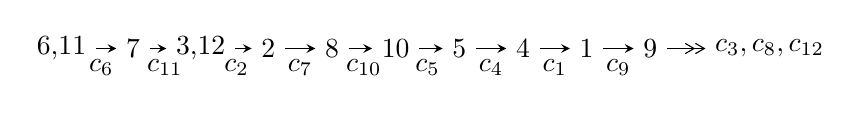
\begin{tikzpicture}[x=23pt, y=7pt]
	% node
	\node (A0) at (-1/8, 0) {6,11};
	\node (A1) at (1, 0) {7};
	\node (A2) at (33/16, 0) {3,12};
	\node (A3) at (25/8, 0) {2};
	\node (A4) at (33/8, 0) {8};
	\node (A5) at (41/8, 0) {10};
	\node (A6) at (49/8, 0) {5};
	\node (A7) at (57/8, 0) {4};
	\node (A8) at (65/8, 0) {1};
	\node (A9) at (73/8, 0) {9};
	\node (C1) at (1/2, -1) {$c_{6}$};
	\node (C2) at (3/2, -1) {$c_{11}$};
	\node (C3) at (21/8, -1) {$c_{2}$};
	\node (C4) at (29/8, -1) {$c_{7}$};
	\node (C5) at (37/8, -1) {$c_{10}$};
	\node (C6) at (45/8, -1) {$c_{5}$};
	\node (C7) at (53/8, -1) {$c_{4}$};
	\node (C8) at (61/8, -1) {$c_{1}$};
	\node (C9) at (69/8, -1) {$c_{9}$};
	\node (A10) at (11, 0) {$c_{3},c_{8},c_{12}$};

	% edge
	\draw[->,>=stealth]	
	(A0) edge (A1) (A1) edge (A2) (A2) edge (A3) (A3) edge (A4) (A4) edge (A5) (A5) edge (A6) (A6) edge (A7) (A7) edge (A8) (A8) edge (A9) ;
	\draw[->>,>={angle 60}]	
	(A9) edge (A10);
\end{tikzpicture} \\ 

\end{tabular} \\

\footnotetext{
The image of knot diagram is generated by the software ``\textbf{Draw programme}" developed by Andrew Bartholomew(\url{http://www.layer8.co.uk/maths/draw/index.htm\#Running-draw}), where we modified some parts for our purpose(\url{https://github.com/CATsTAILs/LinksPainter}).
}\phantom \\ \newline 
\centering \textbf{Ideals for irreducible components\footnotemark of $X_{\text{par}}$} 
 
\begin{align*}
I^u_{1}&=\langle 
4.86488\times10^{164} u^{74}+2.61870\times10^{164} u^{73}+\cdots+7.00921\times10^{164} b+5.62454\times10^{165},\\
\phantom{I^u_{1}}&\phantom{= \langle  }1.09347\times10^{165} u^{74}+1.00292\times10^{165} u^{73}+\cdots+2.10276\times10^{165} a+1.21416\times10^{166},\\
\phantom{I^u_{1}}&\phantom{= \langle  }u^{75}-26 u^{73}+\cdots-29 u-11\rangle \\
I^u_{2}&=\langle 
3565784 u^{20}+1758543 u^{19}+\cdots+4587301 b+16185776,\\
\phantom{I^u_{2}}&\phantom{= \langle  }-848187 u^{20}+33456238 u^{19}+\cdots+22936505 a-154067073,\;u^{21}+u^{20}+\cdots-6 u+5\rangle \\
\\
\end{align*}
\raggedright * 2 irreducible components of $\dim_{\mathbb{C}}=0$, with total 96 representations.\\
\footnotetext{All coefficients of polynomials are rational numbers. But the coefficients are sometimes approximated in decimal forms when there is not enough margin.}
\newpage
\renewcommand{\arraystretch}{1}
\centering \section*{I. $I^u_{1}= \langle 4.86\times10^{164} u^{74}+2.62\times10^{164} u^{73}+\cdots+7.01\times10^{164} b+5.62\times10^{165},\;1.09\times10^{165} u^{74}+1.00\times10^{165} u^{73}+\cdots+2.10\times10^{165} a+1.21\times10^{166},\;u^{75}-26 u^{73}+\cdots-29 u-11 \rangle$}
\flushleft \textbf{(i) Arc colorings}\\
\begin{tabular}{m{7pt} m{180pt} m{7pt} m{180pt} }
\flushright $a_{6}=$&$\begin{pmatrix}1\\0\end{pmatrix}$ \\
\flushright $a_{11}=$&$\begin{pmatrix}0\\u\end{pmatrix}$ \\
\flushright $a_{7}=$&$\begin{pmatrix}1\\- u^2\end{pmatrix}$ \\
\flushright $a_{3}=$&$\begin{pmatrix}-0.520016 u^{74}-0.476954 u^{73}+\cdots+17.4523 u-5.77412\\-0.694069 u^{74}-0.373608 u^{73}+\cdots-32.7082 u-8.02450\end{pmatrix}$ \\
\flushright $a_{12}=$&$\begin{pmatrix}u\\- u^3+u\end{pmatrix}$ \\
\flushright $a_{2}=$&$\begin{pmatrix}0.174054 u^{74}-0.103346 u^{73}+\cdots+50.1605 u+2.25038\\-0.694069 u^{74}-0.373608 u^{73}+\cdots-32.7082 u-8.02450\end{pmatrix}$ \\
\flushright $a_{8}=$&$\begin{pmatrix}0.492874 u^{74}+0.989732 u^{73}+\cdots+37.5192 u+6.43908\\-0.533362 u^{74}-0.574794 u^{73}+\cdots-25.1238 u-7.74220\end{pmatrix}$ \\
\flushright $a_{10}=$&$\begin{pmatrix}0.232330 u^{74}+0.157784 u^{73}+\cdots+85.2464 u+7.12576\\0.332393 u^{74}+0.264914 u^{73}+\cdots+8.68473 u+1.62379\end{pmatrix}$ \\
\flushright $a_{5}=$&$\begin{pmatrix}0.118936 u^{74}-0.271370 u^{73}+\cdots+78.1808 u+7.39601\\0.581180 u^{74}+0.461009 u^{73}+\cdots+26.2919 u+6.63202\end{pmatrix}$ \\
\flushright $a_{4}=$&$\begin{pmatrix}-0.0260069 u^{74}-0.241627 u^{73}+\cdots+43.5597 u-0.0222318\\-0.483810 u^{74}-0.266665 u^{73}+\cdots-18.8593 u-4.86120\end{pmatrix}$ \\
\flushright $a_{1}=$&$\begin{pmatrix}-0.608923 u^{74}-0.434802 u^{73}+\cdots-30.3780 u-3.65550\\-0.433540 u^{74}-0.348757 u^{73}+\cdots-25.2954 u-5.66632\end{pmatrix}$ \\
\flushright $a_{9}=$&$\begin{pmatrix}0.194330 u^{74}+0.575188 u^{73}+\cdots+19.9609 u+1.00031\\-0.583866 u^{74}-0.672134 u^{73}+\cdots-27.3764 u-8.62099\end{pmatrix}$\\&\end{tabular}
\flushleft \textbf{(ii) Obstruction class $= -1$}\\~\\
\flushleft \textbf{(iii) Cusp Shapes $= -3.00721 u^{74}-1.40524 u^{73}+\cdots-209.477 u-50.8854$}\\~\\
\newpage\renewcommand{\arraystretch}{1}
\flushleft \textbf{(iv) u-Polynomials at the component}\newline \\
\begin{tabular}{m{50pt}|m{274pt}}
Crossings & \hspace{64pt}u-Polynomials at each crossing \\
\hline $$\begin{aligned}c_{1}\end{aligned}$$&$\begin{aligned}
&u^{75}+4 u^{74}+\cdots+19778 u+1511
\end{aligned}$\\
\hline $$\begin{aligned}c_{2}\end{aligned}$$&$\begin{aligned}
&u^{75}-7 u^{74}+\cdots+18 u+1
\end{aligned}$\\
\hline $$\begin{aligned}c_{3}\end{aligned}$$&$\begin{aligned}
&u^{75}-2 u^{74}+\cdots-264568 u+145247
\end{aligned}$\\
\hline $$\begin{aligned}c_{4}\end{aligned}$$&$\begin{aligned}
&u^{75}+u^{74}+\cdots-4794 u-103
\end{aligned}$\\
\hline $$\begin{aligned}c_{5},c_{9}\end{aligned}$$&$\begin{aligned}
&u^{75}-3 u^{74}+\cdots+4690 u-3812
\end{aligned}$\\
\hline $$\begin{aligned}c_{6},c_{11}\end{aligned}$$&$\begin{aligned}
&u^{75}-26 u^{73}+\cdots-29 u+11
\end{aligned}$\\
\hline $$\begin{aligned}c_{7}\end{aligned}$$&$\begin{aligned}
&u^{75}+u^{74}+\cdots+1531 u-221
\end{aligned}$\\
\hline $$\begin{aligned}c_{8},c_{12}\end{aligned}$$&$\begin{aligned}
&u^{75}-5 u^{74}+\cdots+6535 u+1379
\end{aligned}$\\
\hline $$\begin{aligned}c_{10}\end{aligned}$$&$\begin{aligned}
&u^{75}-2 u^{74}+\cdots-27 u+7
\end{aligned}$\\
\hline
\end{tabular}\\~\\
\newpage\renewcommand{\arraystretch}{1}
\flushleft \textbf{(v) Riley Polynomials at the component}\newline \\
\begin{tabular}{m{50pt}|m{274pt}}
Crossings & \hspace{64pt}Riley Polynomials at each crossing \\
\hline $$\begin{aligned}c_{1}\end{aligned}$$&$\begin{aligned}
&y^{75}+72 y^{74}+\cdots-34177216 y-2283121
\end{aligned}$\\
\hline $$\begin{aligned}c_{2}\end{aligned}$$&$\begin{aligned}
&y^{75}+11 y^{74}+\cdots+92 y-1
\end{aligned}$\\
\hline $$\begin{aligned}c_{3}\end{aligned}$$&$\begin{aligned}
&y^{75}+36 y^{74}+\cdots+220857023174 y-21096691009
\end{aligned}$\\
\hline $$\begin{aligned}c_{4}\end{aligned}$$&$\begin{aligned}
&y^{75}+85 y^{74}+\cdots+17227620 y-10609
\end{aligned}$\\
\hline $$\begin{aligned}c_{5},c_{9}\end{aligned}$$&$\begin{aligned}
&y^{75}-45 y^{74}+\cdots+350201676 y-14531344
\end{aligned}$\\
\hline $$\begin{aligned}c_{6},c_{11}\end{aligned}$$&$\begin{aligned}
&y^{75}-52 y^{74}+\cdots+6627 y-121
\end{aligned}$\\
\hline $$\begin{aligned}c_{7}\end{aligned}$$&$\begin{aligned}
&y^{75}+37 y^{74}+\cdots+884919 y-48841
\end{aligned}$\\
\hline $$\begin{aligned}c_{8},c_{12}\end{aligned}$$&$\begin{aligned}
&y^{75}-87 y^{74}+\cdots+99190065 y-1901641
\end{aligned}$\\
\hline $$\begin{aligned}c_{10}\end{aligned}$$&$\begin{aligned}
&y^{75}+8 y^{74}+\cdots-2407 y-49
\end{aligned}$\\
\hline
\end{tabular}\\~\\
\newpage\flushleft \textbf{(vi) Complex Volumes and Cusp Shapes}
$$\begin{array}{c|c|c}  
\text{Solutions to }I^u_{1}& \I (\text{vol} + \sqrt{-1}CS) & \text{Cusp shape}\\
 \hline 
\begin{aligned}
u &= -0.013866 + 0.992612 I \\
a &= \phantom{-}0.692135 + 0.718908 I \\
b &= \phantom{-}0.400349 + 1.084530 I\end{aligned}
 & -6.17619 + 2.37907 I & \phantom{-0.000000 } 0 \\ \hline\begin{aligned}
u &= -0.013866 - 0.992612 I \\
a &= \phantom{-}0.692135 - 0.718908 I \\
b &= \phantom{-}0.400349 - 1.084530 I\end{aligned}
 & -6.17619 - 2.37907 I & \phantom{-0.000000 } 0 \\ \hline\begin{aligned}
u &= \phantom{-}0.939254 + 0.315999 I \\
a &= \phantom{-}0.018888 + 0.438631 I \\
b &= -0.664173 + 0.848941 I\end{aligned}
 & -1.07144 + 2.44545 I & \phantom{-0.000000 } 0 \\ \hline\begin{aligned}
u &= \phantom{-}0.939254 - 0.315999 I \\
a &= \phantom{-}0.018888 - 0.438631 I \\
b &= -0.664173 - 0.848941 I\end{aligned}
 & -1.07144 - 2.44545 I & \phantom{-0.000000 } 0 \\ \hline\begin{aligned}
u &= -0.938498 + 0.408238 I \\
a &= \phantom{-}0.13100 + 1.90136 I \\
b &= -0.330038 + 0.911612 I\end{aligned}
 & -1.29527 - 3.07415 I & \phantom{-0.000000 } 0 \\ \hline\begin{aligned}
u &= -0.938498 - 0.408238 I \\
a &= \phantom{-}0.13100 - 1.90136 I \\
b &= -0.330038 - 0.911612 I\end{aligned}
 & -1.29527 + 3.07415 I & \phantom{-0.000000 } 0 \\ \hline\begin{aligned}
u &= -0.960972 + 0.048035 I \\
a &= -0.544278 + 1.052270 I \\
b &= \phantom{-}0.903732 + 0.646873 I\end{aligned}
 & \phantom{-}1.079070 - 0.291978 I & \phantom{-0.000000 } 0 \\ \hline\begin{aligned}
u &= -0.960972 - 0.048035 I \\
a &= -0.544278 - 1.052270 I \\
b &= \phantom{-}0.903732 - 0.646873 I\end{aligned}
 & \phantom{-}1.079070 + 0.291978 I & \phantom{-0.000000 } 0 \\ \hline\begin{aligned}
u &= -0.966822 + 0.378367 I \\
a &= \phantom{-}1.94521 - 0.03260 I \\
b &= -0.084333 + 0.363747 I\end{aligned}
 & \phantom{-}2.57495 - 7.43580 I & \phantom{-0.000000 } 0 \\ \hline\begin{aligned}
u &= -0.966822 - 0.378367 I \\
a &= \phantom{-}1.94521 + 0.03260 I \\
b &= -0.084333 - 0.363747 I\end{aligned}
 & \phantom{-}2.57495 + 7.43580 I & \phantom{-0.000000 } 0\\
 \hline 
 \end{array}$$\newpage$$\begin{array}{c|c|c}  
\text{Solutions to }I^u_{1}& \I (\text{vol} + \sqrt{-1}CS) & \text{Cusp shape}\\
 \hline 
\begin{aligned}
u &= -1.034730 + 0.129185 I \\
a &= \phantom{-}0.145476 - 0.953838 I \\
b &= -0.87885 - 1.88423 I\end{aligned}
 & \phantom{-}5.36144 - 1.41166 I & \phantom{-0.000000 } 0 \\ \hline\begin{aligned}
u &= -1.034730 - 0.129185 I \\
a &= \phantom{-}0.145476 + 0.953838 I \\
b &= -0.87885 + 1.88423 I\end{aligned}
 & \phantom{-}5.36144 + 1.41166 I & \phantom{-0.000000 } 0 \\ \hline\begin{aligned}
u &= \phantom{-}0.907268 + 0.075300 I \\
a &= \phantom{-}0.94549 - 2.12345 I \\
b &= -0.523555 - 0.950514 I\end{aligned}
 & -3.93565 + 1.98540 I & \phantom{-0.000000 -}0. + 3.06730 I \\ \hline\begin{aligned}
u &= \phantom{-}0.907268 - 0.075300 I \\
a &= \phantom{-}0.94549 + 2.12345 I \\
b &= -0.523555 + 0.950514 I\end{aligned}
 & -3.93565 - 1.98540 I & \phantom{-0.000000 } 0. - 3.06730 I \\ \hline\begin{aligned}
u &= \phantom{-}1.110880 + 0.165795 I \\
a &= -0.047261 - 0.317334 I \\
b &= \phantom{-}2.14672 - 0.81505 I\end{aligned}
 & \phantom{-}5.56938 + 6.51079 I & \phantom{-0.000000 } 0 \\ \hline\begin{aligned}
u &= \phantom{-}1.110880 - 0.165795 I \\
a &= -0.047261 + 0.317334 I \\
b &= \phantom{-}2.14672 + 0.81505 I\end{aligned}
 & \phantom{-}5.56938 - 6.51079 I & \phantom{-0.000000 } 0 \\ \hline\begin{aligned}
u &= -1.160340 + 0.126685 I \\
a &= \phantom{-}0.282949 + 0.314124 I \\
b &= -0.837413 + 0.239299 I\end{aligned}
 & \phantom{-}2.25915 - 0.14325 I & \phantom{-0.000000 } 0 \\ \hline\begin{aligned}
u &= -1.160340 - 0.126685 I \\
a &= \phantom{-}0.282949 - 0.314124 I \\
b &= -0.837413 - 0.239299 I\end{aligned}
 & \phantom{-}2.25915 + 0.14325 I & \phantom{-0.000000 } 0 \\ \hline\begin{aligned}
u &= \phantom{-}0.206317 + 1.155090 I \\
a &= -0.603459 + 0.707647 I \\
b &= -0.521027 + 0.818222 I\end{aligned}
 & -4.61919 - 3.44875 I & \phantom{-0.000000 } 0 \\ \hline\begin{aligned}
u &= \phantom{-}0.206317 - 1.155090 I \\
a &= -0.603459 - 0.707647 I \\
b &= -0.521027 - 0.818222 I\end{aligned}
 & -4.61919 + 3.44875 I & \phantom{-0.000000 } 0\\
 \hline 
 \end{array}$$\newpage$$\begin{array}{c|c|c}  
\text{Solutions to }I^u_{1}& \I (\text{vol} + \sqrt{-1}CS) & \text{Cusp shape}\\
 \hline 
\begin{aligned}
u &= \phantom{-}1.114000 + 0.368961 I \\
a &= -1.019900 + 0.719651 I \\
b &= \phantom{-}0.988836 + 0.744888 I\end{aligned}
 & \phantom{-}4.35958 + 4.55603 I & \phantom{-0.000000 } 0 \\ \hline\begin{aligned}
u &= \phantom{-}1.114000 - 0.368961 I \\
a &= -1.019900 - 0.719651 I \\
b &= \phantom{-}0.988836 - 0.744888 I\end{aligned}
 & \phantom{-}4.35958 - 4.55603 I & \phantom{-0.000000 } 0 \\ \hline\begin{aligned}
u &= \phantom{-}0.760290 + 0.301132 I \\
a &= -1.63953 - 0.05711 I \\
b &= -0.341483 + 0.350286 I\end{aligned}
 & -3.59837 - 0.23339 I & \phantom{-}3.34922 - 1.64513 I \\ \hline\begin{aligned}
u &= \phantom{-}0.760290 - 0.301132 I \\
a &= -1.63953 + 0.05711 I \\
b &= -0.341483 - 0.350286 I\end{aligned}
 & -3.59837 + 0.23339 I & \phantom{-}3.34922 + 1.64513 I \\ \hline\begin{aligned}
u &= -0.002744 + 1.189670 I \\
a &= \phantom{-}0.701533 - 0.828624 I \\
b &= \phantom{-}0.653223 - 1.002770 I\end{aligned}
 & -0.08499 - 10.49950 I & \phantom{-0.000000 } 0 \\ \hline\begin{aligned}
u &= -0.002744 - 1.189670 I \\
a &= \phantom{-}0.701533 + 0.828624 I \\
b &= \phantom{-}0.653223 + 1.002770 I\end{aligned}
 & -0.08499 + 10.49950 I & \phantom{-0.000000 } 0 \\ \hline\begin{aligned}
u &= \phantom{-}1.172170 + 0.305565 I \\
a &= \phantom{-}0.523471 + 0.816282 I \\
b &= -0.132271 - 0.058421 I\end{aligned}
 & -1.80185 + 2.16906 I & \phantom{-0.000000 } 0 \\ \hline\begin{aligned}
u &= \phantom{-}1.172170 - 0.305565 I \\
a &= \phantom{-}0.523471 - 0.816282 I \\
b &= -0.132271 + 0.058421 I\end{aligned}
 & -1.80185 - 2.16906 I & \phantom{-0.000000 } 0 \\ \hline\begin{aligned}
u &= \phantom{-}1.173800 + 0.362759 I \\
a &= -0.378650 + 0.861125 I \\
b &= \phantom{-}1.099170 + 0.869923 I\end{aligned}
 & \phantom{-}3.34164 + 4.17608 I & \phantom{-0.000000 } 0 \\ \hline\begin{aligned}
u &= \phantom{-}1.173800 - 0.362759 I \\
a &= -0.378650 - 0.861125 I \\
b &= \phantom{-}1.099170 - 0.869923 I\end{aligned}
 & \phantom{-}3.34164 - 4.17608 I & \phantom{-0.000000 } 0\\
 \hline 
 \end{array}$$\newpage$$\begin{array}{c|c|c}  
\text{Solutions to }I^u_{1}& \I (\text{vol} + \sqrt{-1}CS) & \text{Cusp shape}\\
 \hline 
\begin{aligned}
u &= -0.052071 + 0.743666 I \\
a &= -1.22281 - 1.12361 I \\
b &= -0.525972 - 1.114410 I\end{aligned}
 & -6.07542 + 3.12385 I & -2.56319 - 4.01706 I \\ \hline\begin{aligned}
u &= -0.052071 - 0.743666 I \\
a &= -1.22281 + 1.12361 I \\
b &= -0.525972 + 1.114410 I\end{aligned}
 & -6.07542 - 3.12385 I & -2.56319 + 4.01706 I \\ \hline\begin{aligned}
u &= \phantom{-}0.647746 + 0.356319 I \\
a &= -0.52809 + 1.45131 I \\
b &= \phantom{-}1.33036 + 0.69475 I\end{aligned}
 & \phantom{-}3.40846 + 5.43996 I & -0.90178 - 5.14570 I \\ \hline\begin{aligned}
u &= \phantom{-}0.647746 - 0.356319 I \\
a &= -0.52809 - 1.45131 I \\
b &= \phantom{-}1.33036 - 0.69475 I\end{aligned}
 & \phantom{-}3.40846 - 5.43996 I & -0.90178 + 5.14570 I \\ \hline\begin{aligned}
u &= -1.237780 + 0.300983 I \\
a &= -0.68099 - 1.37162 I \\
b &= \phantom{-}0.955357 - 0.902724 I\end{aligned}
 & \phantom{-}7.74101 - 8.12655 I & \phantom{-0.000000 } 0 \\ \hline\begin{aligned}
u &= -1.237780 - 0.300983 I \\
a &= -0.68099 + 1.37162 I \\
b &= \phantom{-}0.955357 + 0.902724 I\end{aligned}
 & \phantom{-}7.74101 + 8.12655 I & \phantom{-0.000000 } 0 \\ \hline\begin{aligned}
u &= -0.404055 + 0.594522 I \\
a &= \phantom{-}0.79451 - 1.92548 I \\
b &= \phantom{-}0.006207 - 1.108050 I\end{aligned}
 & \phantom{-}1.03252 + 3.60544 I & -4.06380 - 1.82140 I \\ \hline\begin{aligned}
u &= -0.404055 - 0.594522 I \\
a &= \phantom{-}0.79451 + 1.92548 I \\
b &= \phantom{-}0.006207 + 1.108050 I\end{aligned}
 & \phantom{-}1.03252 - 3.60544 I & -4.06380 + 1.82140 I \\ \hline\begin{aligned}
u &= \phantom{-}0.686004\phantom{ +0.000000I} \\
a &= \phantom{-}1.77921\phantom{ +0.000000I} \\
b &= -1.18115\phantom{ +0.000000I}\end{aligned}
 & -2.50904\phantom{ +0.000000I} & -13.2560\phantom{ +0.000000I} \\ \hline\begin{aligned}
u &= -1.337960 + 0.048610 I \\
a &= \phantom{-}0.085328 + 0.223266 I \\
b &= \phantom{-}0.89019 + 1.54950 I\end{aligned}
 & \phantom{-}6.53570 - 1.10775 I & \phantom{-0.000000 } 0\\
 \hline 
 \end{array}$$\newpage$$\begin{array}{c|c|c}  
\text{Solutions to }I^u_{1}& \I (\text{vol} + \sqrt{-1}CS) & \text{Cusp shape}\\
 \hline 
\begin{aligned}
u &= -1.337960 - 0.048610 I \\
a &= \phantom{-}0.085328 - 0.223266 I \\
b &= \phantom{-}0.89019 - 1.54950 I\end{aligned}
 & \phantom{-}6.53570 + 1.10775 I & \phantom{-0.000000 } 0 \\ \hline\begin{aligned}
u &= -1.278100 + 0.422698 I \\
a &= \phantom{-}0.395219 + 1.012020 I \\
b &= -1.09039 + 1.47215 I\end{aligned}
 & -2.27515 - 7.48919 I & \phantom{-0.000000 } 0 \\ \hline\begin{aligned}
u &= -1.278100 - 0.422698 I \\
a &= \phantom{-}0.395219 - 1.012020 I \\
b &= -1.09039 - 1.47215 I\end{aligned}
 & -2.27515 + 7.48919 I & \phantom{-0.000000 } 0 \\ \hline\begin{aligned}
u &= -0.630165 + 0.173633 I \\
a &= \phantom{-}1.17934 - 1.10273 I \\
b &= -0.690665 + 0.543583 I\end{aligned}
 & \phantom{-}4.27365 - 0.04437 I & \phantom{-}3.14115 + 2.61297 I \\ \hline\begin{aligned}
u &= -0.630165 - 0.173633 I \\
a &= \phantom{-}1.17934 + 1.10273 I \\
b &= -0.690665 - 0.543583 I\end{aligned}
 & \phantom{-}4.27365 + 0.04437 I & \phantom{-}3.14115 - 2.61297 I \\ \hline\begin{aligned}
u &= \phantom{-}0.201905 + 0.589482 I \\
a &= \phantom{-}0.41957 - 1.35572 I \\
b &= \phantom{-}0.678636 - 1.018540 I\end{aligned}
 & \phantom{-}1.71568 - 0.87377 I & -4.45101 - 0.59244 I \\ \hline\begin{aligned}
u &= \phantom{-}0.201905 - 0.589482 I \\
a &= \phantom{-}0.41957 + 1.35572 I \\
b &= \phantom{-}0.678636 + 1.018540 I\end{aligned}
 & \phantom{-}1.71568 + 0.87377 I & -4.45101 + 0.59244 I \\ \hline\begin{aligned}
u &= \phantom{-}1.255700 + 0.619721 I \\
a &= \phantom{-}0.150657 - 0.302176 I \\
b &= -0.850030 - 0.371842 I\end{aligned}
 & -1.71673 + 3.48360 I & \phantom{-0.000000 } 0 \\ \hline\begin{aligned}
u &= \phantom{-}1.255700 - 0.619721 I \\
a &= \phantom{-}0.150657 + 0.302176 I \\
b &= -0.850030 + 0.371842 I\end{aligned}
 & -1.71673 - 3.48360 I & \phantom{-0.000000 } 0 \\ \hline\begin{aligned}
u &= \phantom{-}1.373600 + 0.302564 I \\
a &= \phantom{-}0.148834 - 0.958574 I \\
b &= -0.831950 - 0.610118 I\end{aligned}
 & \phantom{-}11.26350 + 2.23040 I & \phantom{-0.000000 } 0\\
 \hline 
 \end{array}$$\newpage$$\begin{array}{c|c|c}  
\text{Solutions to }I^u_{1}& \I (\text{vol} + \sqrt{-1}CS) & \text{Cusp shape}\\
 \hline 
\begin{aligned}
u &= \phantom{-}1.373600 - 0.302564 I \\
a &= \phantom{-}0.148834 + 0.958574 I \\
b &= -0.831950 + 0.610118 I\end{aligned}
 & \phantom{-}11.26350 - 2.23040 I & \phantom{-0.000000 } 0 \\ \hline\begin{aligned}
u &= \phantom{-}1.277590 + 0.602915 I \\
a &= \phantom{-}0.361233 - 1.084430 I \\
b &= -1.00616 - 1.06220 I\end{aligned}
 & -1.23702 + 9.55268 I & \phantom{-0.000000 } 0 \\ \hline\begin{aligned}
u &= \phantom{-}1.277590 - 0.602915 I \\
a &= \phantom{-}0.361233 + 1.084430 I \\
b &= -1.00616 + 1.06220 I\end{aligned}
 & -1.23702 - 9.55268 I & \phantom{-0.000000 } 0 \\ \hline\begin{aligned}
u &= -0.53023 + 1.32146 I \\
a &= -0.371566 + 0.232025 I \\
b &= -0.602848 - 0.069339 I\end{aligned}
 & \phantom{-}4.94966 + 2.13138 I & \phantom{-0.000000 } 0 \\ \hline\begin{aligned}
u &= -0.53023 - 1.32146 I \\
a &= -0.371566 - 0.232025 I \\
b &= -0.602848 + 0.069339 I\end{aligned}
 & \phantom{-}4.94966 - 2.13138 I & \phantom{-0.000000 } 0 \\ \hline\begin{aligned}
u &= -1.33869 + 0.49079 I \\
a &= -0.297532 - 0.830875 I \\
b &= \phantom{-}1.12359 - 1.40728 I\end{aligned}
 & -2.01665 - 7.67344 I & \phantom{-0.000000 } 0 \\ \hline\begin{aligned}
u &= -1.33869 - 0.49079 I \\
a &= -0.297532 + 0.830875 I \\
b &= \phantom{-}1.12359 + 1.40728 I\end{aligned}
 & -2.01665 + 7.67344 I & \phantom{-0.000000 } 0 \\ \hline\begin{aligned}
u &= \phantom{-}1.43679 + 0.09756 I \\
a &= -0.060747 + 0.750626 I \\
b &= \phantom{-}0.00253 + 2.18189 I\end{aligned}
 & \phantom{-}7.07352 - 1.46642 I & \phantom{-0.000000 } 0 \\ \hline\begin{aligned}
u &= \phantom{-}1.43679 - 0.09756 I \\
a &= -0.060747 - 0.750626 I \\
b &= \phantom{-}0.00253 - 2.18189 I\end{aligned}
 & \phantom{-}7.07352 + 1.46642 I & \phantom{-0.000000 } 0 \\ \hline\begin{aligned}
u &= \phantom{-}1.04085 + 1.02337 I \\
a &= \phantom{-}0.404301 + 0.100962 I \\
b &= \phantom{-}0.686049 - 0.445349 I\end{aligned}
 & \phantom{-}3.77545 + 0.13140 I & \phantom{-0.000000 } 0\\
 \hline 
 \end{array}$$\newpage$$\begin{array}{c|c|c}  
\text{Solutions to }I^u_{1}& \I (\text{vol} + \sqrt{-1}CS) & \text{Cusp shape}\\
 \hline 
\begin{aligned}
u &= \phantom{-}1.04085 - 1.02337 I \\
a &= \phantom{-}0.404301 - 0.100962 I \\
b &= \phantom{-}0.686049 + 0.445349 I\end{aligned}
 & \phantom{-}3.77545 - 0.13140 I & \phantom{-0.000000 } 0 \\ \hline\begin{aligned}
u &= -0.520472\phantom{ +0.000000I} \\
a &= -3.56024\phantom{ +0.000000I} \\
b &= -0.196479\phantom{ +0.000000I}\end{aligned}
 & -2.81755\phantom{ +0.000000I} & -5.84520\phantom{ +0.000000I} \\ \hline\begin{aligned}
u &= \phantom{-}1.37763 + 0.57274 I \\
a &= -0.327901 + 1.049300 I \\
b &= \phantom{-}1.16712 + 1.26375 I\end{aligned}
 & \phantom{-}4.2230 + 16.6469 I & \phantom{-0.000000 } 0 \\ \hline\begin{aligned}
u &= \phantom{-}1.37763 - 0.57274 I \\
a &= -0.327901 - 1.049300 I \\
b &= \phantom{-}1.16712 - 1.26375 I\end{aligned}
 & \phantom{-}4.2230 - 16.6469 I & \phantom{-0.000000 } 0 \\ \hline\begin{aligned}
u &= -1.29659 + 0.76159 I \\
a &= -0.040832 - 0.596066 I \\
b &= \phantom{-}0.645843 - 0.482141 I\end{aligned}
 & \phantom{-}0.41911 - 3.99968 I & \phantom{-0.000000 } 0 \\ \hline\begin{aligned}
u &= -1.29659 - 0.76159 I \\
a &= -0.040832 + 0.596066 I \\
b &= \phantom{-}0.645843 + 0.482141 I\end{aligned}
 & \phantom{-}0.41911 + 3.99968 I & \phantom{-0.000000 } 0 \\ \hline\begin{aligned}
u &= -1.37317 + 0.63897 I \\
a &= \phantom{-}0.030652 + 0.763246 I \\
b &= -1.163710 + 0.673853 I\end{aligned}
 & \phantom{-}8.47631 - 9.19794 I & \phantom{-0.000000 } 0 \\ \hline\begin{aligned}
u &= -1.37317 - 0.63897 I \\
a &= \phantom{-}0.030652 - 0.763246 I \\
b &= -1.163710 - 0.673853 I\end{aligned}
 & \phantom{-}8.47631 + 9.19794 I & \phantom{-0.000000 } 0 \\ \hline\begin{aligned}
u &= \phantom{-}0.399944 + 0.225942 I \\
a &= -0.97127 + 2.25690 I \\
b &= \phantom{-}1.265320 + 0.451196 I\end{aligned}
 & \phantom{-}3.42078 + 5.42017 I & -0.67147 - 4.81273 I \\ \hline\begin{aligned}
u &= \phantom{-}0.399944 - 0.225942 I \\
a &= -0.97127 - 2.25690 I \\
b &= \phantom{-}1.265320 - 0.451196 I\end{aligned}
 & \phantom{-}3.42078 - 5.42017 I & -0.67147 + 4.81273 I\\
 \hline 
 \end{array}$$\newpage$$\begin{array}{c|c|c}  
\text{Solutions to }I^u_{1}& \I (\text{vol} + \sqrt{-1}CS) & \text{Cusp shape}\\
 \hline 
\begin{aligned}
u &= -0.047641 + 0.411386 I \\
a &= \phantom{-}1.018950 - 0.899310 I \\
b &= \phantom{-}0.382640 - 0.474799 I\end{aligned}
 & -0.012233 - 1.006120 I & -0.14669 + 6.62242 I \\ \hline\begin{aligned}
u &= -0.047641 - 0.411386 I \\
a &= \phantom{-}1.018950 + 0.899310 I \\
b &= \phantom{-}0.382640 + 0.474799 I\end{aligned}
 & -0.012233 + 1.006120 I & -0.14669 - 6.62242 I \\ \hline\begin{aligned}
u &= -0.167122\phantom{ +0.000000I} \\
a &= -8.32002\phantom{ +0.000000I} \\
b &= -0.479306\phantom{ +0.000000I}\end{aligned}
 & -2.84829\phantom{ +0.000000I} & -2.66050\phantom{ +0.000000I} \\ \hline\begin{aligned}
u &= -1.79051 + 0.67497 I \\
a &= \phantom{-}0.228770 - 0.140811 I \\
b &= \phantom{-}0.177471 + 0.154132 I\end{aligned}
 & \phantom{-}4.72272 + 3.49376 I & \phantom{-0.000000 } 0 \\ \hline\begin{aligned}
u &= -1.79051 - 0.67497 I \\
a &= \phantom{-}0.228770 + 0.140811 I \\
b &= \phantom{-}0.177471 - 0.154132 I\end{aligned}
 & \phantom{-}4.72272 - 3.49376 I & \phantom{-0.000000 } 0\\
 \hline 
 \end{array}$$\newpage\newpage\renewcommand{\arraystretch}{1}
\centering \section*{II. $I^u_{2}= \langle 3.57\times10^{6} u^{20}+1.76\times10^{6} u^{19}+\cdots+4.59\times10^{6} b+1.62\times10^{7},\;-8.48\times10^{5} u^{20}+3.35\times10^{7} u^{19}+\cdots+2.29\times10^{7} a-1.54\times10^{8},\;u^{21}+u^{20}+\cdots-6 u+5 \rangle$}
\flushleft \textbf{(i) Arc colorings}\\
\begin{tabular}{m{7pt} m{180pt} m{7pt} m{180pt} }
\flushright $a_{6}=$&$\begin{pmatrix}1\\0\end{pmatrix}$ \\
\flushright $a_{11}=$&$\begin{pmatrix}0\\u\end{pmatrix}$ \\
\flushright $a_{7}=$&$\begin{pmatrix}1\\- u^2\end{pmatrix}$ \\
\flushright $a_{3}=$&$\begin{pmatrix}0.0369798 u^{20}-1.45865 u^{19}+\cdots-13.1245 u+6.71711\\-0.777316 u^{20}-0.383350 u^{19}+\cdots+6.41390 u-3.52839\end{pmatrix}$ \\
\flushright $a_{12}=$&$\begin{pmatrix}u\\- u^3+u\end{pmatrix}$ \\
\flushright $a_{2}=$&$\begin{pmatrix}0.814296 u^{20}-1.07530 u^{19}+\cdots-19.5384 u+10.2455\\-0.777316 u^{20}-0.383350 u^{19}+\cdots+6.41390 u-3.52839\end{pmatrix}$ \\
\flushright $a_{8}=$&$\begin{pmatrix}-0.252921 u^{20}-0.758060 u^{19}+\cdots-2.49621 u+5.84126\\-0.495626 u^{20}-0.795075 u^{19}+\cdots+1.93899 u+0.815101\end{pmatrix}$ \\
\flushright $a_{10}=$&$\begin{pmatrix}0.860543 u^{20}+1.73551 u^{19}+\cdots+11.3000 u-9.27095\\0.326407 u^{20}+0.988228 u^{19}+\cdots+1.22673 u-2.67701\end{pmatrix}$ \\
\flushright $a_{5}=$&$\begin{pmatrix}0.00585499 u^{20}-0.951995 u^{19}+\cdots-14.0920 u+3.66552\\0.210010 u^{20}+0.171345 u^{19}+\cdots+0.699044 u-2.11466\end{pmatrix}$ \\
\flushright $a_{4}=$&$\begin{pmatrix}0.965535 u^{20}-1.09140 u^{19}+\cdots-22.6790 u+10.0385\\-0.611923 u^{20}-0.730373 u^{19}+\cdots+4.87009 u-3.01351\end{pmatrix}$ \\
\flushright $a_{1}=$&$\begin{pmatrix}-0.244683 u^{20}-0.311053 u^{19}+\cdots-2.38142 u+3.17549\\-0.128348 u^{20}-0.518938 u^{19}+\cdots+0.357854 u+0.856290\end{pmatrix}$ \\
\flushright $a_{9}=$&$\begin{pmatrix}-0.422140 u^{20}-0.564907 u^{19}+\cdots+0.669517 u+2.97935\\-0.534291 u^{20}-0.622926 u^{19}+\cdots+2.08439 u-0.234950\end{pmatrix}$\\&\end{tabular}
\flushleft \textbf{(ii) Obstruction class $= 1$}\\~\\
\flushleft \textbf{(iii) Cusp Shapes $= -\frac{2314838}{4587301} u^{20}-\frac{20496911}{4587301} u^{19}+\cdots-\frac{242100829}{4587301} u+\frac{93801989}{4587301}$}\\~\\
\newpage\renewcommand{\arraystretch}{1}
\flushleft \textbf{(iv) u-Polynomials at the component}\newline \\
\begin{tabular}{m{50pt}|m{274pt}}
Crossings & \hspace{64pt}u-Polynomials at each crossing \\
\hline $$\begin{aligned}c_{1}\end{aligned}$$&$\begin{aligned}
&u^{21}-5 u^{20}+\cdots-3 u-1
\end{aligned}$\\
\hline $$\begin{aligned}c_{2}\end{aligned}$$&$\begin{aligned}
&u^{21}+5 u^{19}+\cdots+u-1
\end{aligned}$\\
\hline $$\begin{aligned}c_{3}\end{aligned}$$&$\begin{aligned}
&u^{21}-3 u^{20}+\cdots+47 u+43
\end{aligned}$\\
\hline $$\begin{aligned}c_{4}\end{aligned}$$&$\begin{aligned}
&u^{21}+6 u^{19}+\cdots+7 u+1
\end{aligned}$\\
\hline $$\begin{aligned}c_{5}\end{aligned}$$&$\begin{aligned}
&u^{21}-9 u^{19}+\cdots-10 u-4
\end{aligned}$\\
\hline $$\begin{aligned}c_{6}\end{aligned}$$&$\begin{aligned}
&u^{21}+u^{20}+\cdots-6 u+5
\end{aligned}$\\
\hline $$\begin{aligned}c_{7}\end{aligned}$$&$\begin{aligned}
&u^{21}+8 u^{19}+\cdots-6 u-7
\end{aligned}$\\
\hline $$\begin{aligned}c_{8}\end{aligned}$$&$\begin{aligned}
&u^{21}-8 u^{19}+\cdots+4 u-1
\end{aligned}$\\
\hline $$\begin{aligned}c_{9}\end{aligned}$$&$\begin{aligned}
&u^{21}-9 u^{19}+\cdots-10 u+4
\end{aligned}$\\
\hline $$\begin{aligned}c_{10}\end{aligned}$$&$\begin{aligned}
&u^{21}- u^{20}+\cdots+4 u-1
\end{aligned}$\\
\hline $$\begin{aligned}c_{11}\end{aligned}$$&$\begin{aligned}
&u^{21}- u^{20}+\cdots-6 u-5
\end{aligned}$\\
\hline $$\begin{aligned}c_{12}\end{aligned}$$&$\begin{aligned}
&u^{21}-8 u^{19}+\cdots+4 u+1
\end{aligned}$\\
\hline
\end{tabular}\\~\\
\newpage\renewcommand{\arraystretch}{1}
\flushleft \textbf{(v) Riley Polynomials at the component}\newline \\
\begin{tabular}{m{50pt}|m{274pt}}
Crossings & \hspace{64pt}Riley Polynomials at each crossing \\
\hline $$\begin{aligned}c_{1}\end{aligned}$$&$\begin{aligned}
&y^{21}+11 y^{20}+\cdots+11 y-1
\end{aligned}$\\
\hline $$\begin{aligned}c_{2}\end{aligned}$$&$\begin{aligned}
&y^{21}+10 y^{20}+\cdots-5 y-1
\end{aligned}$\\
\hline $$\begin{aligned}c_{3}\end{aligned}$$&$\begin{aligned}
&y^{21}+27 y^{20}+\cdots+11153 y-1849
\end{aligned}$\\
\hline $$\begin{aligned}c_{4}\end{aligned}$$&$\begin{aligned}
&y^{21}+12 y^{20}+\cdots-17 y-1
\end{aligned}$\\
\hline $$\begin{aligned}c_{5},c_{9}\end{aligned}$$&$\begin{aligned}
&y^{21}-18 y^{20}+\cdots+268 y-16
\end{aligned}$\\
\hline $$\begin{aligned}c_{6},c_{11}\end{aligned}$$&$\begin{aligned}
&y^{21}-17 y^{20}+\cdots+226 y-25
\end{aligned}$\\
\hline $$\begin{aligned}c_{7}\end{aligned}$$&$\begin{aligned}
&y^{21}+16 y^{20}+\cdots-370 y-49
\end{aligned}$\\
\hline $$\begin{aligned}c_{8},c_{12}\end{aligned}$$&$\begin{aligned}
&y^{21}-16 y^{20}+\cdots-20 y-1
\end{aligned}$\\
\hline $$\begin{aligned}c_{10}\end{aligned}$$&$\begin{aligned}
&y^{21}+3 y^{20}+\cdots-4 y-1
\end{aligned}$\\
\hline
\end{tabular}\\~\\
\newpage\flushleft \textbf{(vi) Complex Volumes and Cusp Shapes}
$$\begin{array}{c|c|c}  
\text{Solutions to }I^u_{2}& \I (\text{vol} + \sqrt{-1}CS) & \text{Cusp shape}\\
 \hline 
\begin{aligned}
u &= -1.001020 + 0.262420 I \\
a &= -0.921736 - 0.575279 I \\
b &= \phantom{-}1.64460 - 0.25263 I\end{aligned}
 & \phantom{-}4.36516 - 6.59975 I & \phantom{-}1.05252 + 8.07459 I \\ \hline\begin{aligned}
u &= -1.001020 - 0.262420 I \\
a &= -0.921736 + 0.575279 I \\
b &= \phantom{-}1.64460 + 0.25263 I\end{aligned}
 & \phantom{-}4.36516 + 6.59975 I & \phantom{-}1.05252 - 8.07459 I \\ \hline\begin{aligned}
u &= -0.137847 + 0.949067 I \\
a &= -0.852631 - 0.775856 I \\
b &= -0.503361 - 1.102010 I\end{aligned}
 & -7.38286 + 2.58162 I & -9.14346 - 2.28449 I \\ \hline\begin{aligned}
u &= -0.137847 - 0.949067 I \\
a &= -0.852631 + 0.775856 I \\
b &= -0.503361 + 1.102010 I\end{aligned}
 & -7.38286 - 2.58162 I & -9.14346 + 2.28449 I \\ \hline\begin{aligned}
u &= \phantom{-}0.933976 + 0.190871 I \\
a &= \phantom{-}0.53801 - 2.33404 I \\
b &= -0.338970 - 0.954357 I\end{aligned}
 & -3.93389 + 2.54020 I & -4.26332 - 10.43284 I \\ \hline\begin{aligned}
u &= \phantom{-}0.933976 - 0.190871 I \\
a &= \phantom{-}0.53801 + 2.33404 I \\
b &= -0.338970 + 0.954357 I\end{aligned}
 & -3.93389 - 2.54020 I & -4.26332 + 10.43284 I \\ \hline\begin{aligned}
u &= -0.983637 + 0.420576 I \\
a &= \phantom{-}0.057658 - 0.984094 I \\
b &= \phantom{-}0.000605 - 0.667761 I\end{aligned}
 & -0.01096 - 2.31575 I & \phantom{-}2.89116 + 3.13951 I \\ \hline\begin{aligned}
u &= -0.983637 - 0.420576 I \\
a &= \phantom{-}0.057658 + 0.984094 I \\
b &= \phantom{-}0.000605 + 0.667761 I\end{aligned}
 & -0.01096 + 2.31575 I & \phantom{-}2.89116 - 3.13951 I \\ \hline\begin{aligned}
u &= \phantom{-}0.686384 + 0.325532 I \\
a &= -2.10424 + 0.04632 I \\
b &= -0.267232 + 0.305573 I\end{aligned}
 & -4.27917 - 0.25341 I & -10.22146 - 1.60946 I \\ \hline\begin{aligned}
u &= \phantom{-}0.686384 - 0.325532 I \\
a &= -2.10424 - 0.04632 I \\
b &= -0.267232 - 0.305573 I\end{aligned}
 & -4.27917 + 0.25341 I & -10.22146 + 1.60946 I\\
 \hline 
 \end{array}$$\newpage$$\begin{array}{c|c|c}  
\text{Solutions to }I^u_{2}& \I (\text{vol} + \sqrt{-1}CS) & \text{Cusp shape}\\
 \hline 
\begin{aligned}
u &= -0.753934\phantom{ +0.000000I} \\
a &= \phantom{-}2.10025\phantom{ +0.000000I} \\
b &= -0.921449\phantom{ +0.000000I}\end{aligned}
 & -2.13830\phantom{ +0.000000I} & \phantom{-}10.8270\phantom{ +0.000000I} \\ \hline\begin{aligned}
u &= \phantom{-}0.476315 + 0.539233 I \\
a &= -0.302885 - 0.739305 I \\
b &= -0.310507 + 0.873261 I\end{aligned}
 & \phantom{-}3.63985 + 1.20269 I & \phantom{-}0.11227 - 2.52581 I \\ \hline\begin{aligned}
u &= \phantom{-}0.476315 - 0.539233 I \\
a &= -0.302885 + 0.739305 I \\
b &= -0.310507 - 0.873261 I\end{aligned}
 & \phantom{-}3.63985 - 1.20269 I & \phantom{-}0.11227 + 2.52581 I \\ \hline\begin{aligned}
u &= \phantom{-}1.370620 + 0.034901 I \\
a &= -0.117613 - 0.704260 I \\
b &= \phantom{-}0.02178 - 2.18523 I\end{aligned}
 & \phantom{-}7.55445 + 0.17379 I & \phantom{-}6.36834 + 1.10559 I \\ \hline\begin{aligned}
u &= \phantom{-}1.370620 - 0.034901 I \\
a &= -0.117613 + 0.704260 I \\
b &= \phantom{-}0.02178 + 2.18523 I\end{aligned}
 & \phantom{-}7.55445 - 0.17379 I & \phantom{-}6.36834 - 1.10559 I \\ \hline\begin{aligned}
u &= -1.314580 + 0.500777 I \\
a &= \phantom{-}0.351230 + 0.955966 I \\
b &= -1.05469 + 1.43008 I\end{aligned}
 & -3.61843 - 7.80961 I & -5.08756 + 5.98059 I \\ \hline\begin{aligned}
u &= -1.314580 - 0.500777 I \\
a &= \phantom{-}0.351230 - 0.955966 I \\
b &= -1.05469 - 1.43008 I\end{aligned}
 & -3.61843 + 7.80961 I & -5.08756 - 5.98059 I \\ \hline\begin{aligned}
u &= \phantom{-}1.31032 + 0.74608 I \\
a &= -0.083874 + 0.426133 I \\
b &= \phantom{-}0.761324 + 0.466956 I\end{aligned}
 & -1.66929 + 3.96809 I & -0.71858 - 12.39534 I \\ \hline\begin{aligned}
u &= \phantom{-}1.31032 - 0.74608 I \\
a &= -0.083874 - 0.426133 I \\
b &= \phantom{-}0.761324 - 0.466956 I\end{aligned}
 & -1.66929 - 3.96809 I & -0.71858 + 12.39534 I \\ \hline\begin{aligned}
u &= -1.46356 + 0.64846 I \\
a &= \phantom{-}0.185956 - 0.063411 I \\
b &= \phantom{-}0.507174 - 0.292801 I\end{aligned}
 & \phantom{-}4.75936 + 3.16555 I & \phantom{-}4.09678 + 3.29546 I\\
 \hline 
 \end{array}$$\newpage$$\begin{array}{c|c|c}  
\text{Solutions to }I^u_{2}& \I (\text{vol} + \sqrt{-1}CS) & \text{Cusp shape}\\
 \hline 
\begin{aligned}
u &= -1.46356 - 0.64846 I \\
a &= \phantom{-}0.185956 + 0.063411 I \\
b &= \phantom{-}0.507174 + 0.292801 I\end{aligned}
 & \phantom{-}4.75936 - 3.16555 I & \phantom{-}4.09678 - 3.29546 I\\
 \hline 
 \end{array}$$\newpage
\newpage\renewcommand{\arraystretch}{1}
\centering \section*{ III. u-Polynomials}
\begin{tabular}{m{50pt}|m{274pt}}
Crossings & \hspace{64pt}u-Polynomials at each crossing \\
\hline $$\begin{aligned}c_{1}\end{aligned}$$&$\begin{aligned}
&(u^{21}-5 u^{20}+\cdots-3 u-1)(u^{75}+4 u^{74}+\cdots+19778 u+1511)
\end{aligned}$\\
\hline $$\begin{aligned}c_{2}\end{aligned}$$&$\begin{aligned}
&(u^{21}+5 u^{19}+\cdots+u-1)(u^{75}-7 u^{74}+\cdots+18 u+1)
\end{aligned}$\\
\hline $$\begin{aligned}c_{3}\end{aligned}$$&$\begin{aligned}
&(u^{21}-3 u^{20}+\cdots+47 u+43)(u^{75}-2 u^{74}+\cdots-264568 u+145247)
\end{aligned}$\\
\hline $$\begin{aligned}c_{4}\end{aligned}$$&$\begin{aligned}
&(u^{21}+6 u^{19}+\cdots+7 u+1)(u^{75}+u^{74}+\cdots-4794 u-103)
\end{aligned}$\\
\hline $$\begin{aligned}c_{5}\end{aligned}$$&$\begin{aligned}
&(u^{21}-9 u^{19}+\cdots-10 u-4)(u^{75}-3 u^{74}+\cdots+4690 u-3812)
\end{aligned}$\\
\hline $$\begin{aligned}c_{6}\end{aligned}$$&$\begin{aligned}
&(u^{21}+u^{20}+\cdots-6 u+5)(u^{75}-26 u^{73}+\cdots-29 u+11)
\end{aligned}$\\
\hline $$\begin{aligned}c_{7}\end{aligned}$$&$\begin{aligned}
&(u^{21}+8 u^{19}+\cdots-6 u-7)(u^{75}+u^{74}+\cdots+1531 u-221)
\end{aligned}$\\
\hline $$\begin{aligned}c_{8}\end{aligned}$$&$\begin{aligned}
&(u^{21}-8 u^{19}+\cdots+4 u-1)(u^{75}-5 u^{74}+\cdots+6535 u+1379)
\end{aligned}$\\
\hline $$\begin{aligned}c_{9}\end{aligned}$$&$\begin{aligned}
&(u^{21}-9 u^{19}+\cdots-10 u+4)(u^{75}-3 u^{74}+\cdots+4690 u-3812)
\end{aligned}$\\
\hline $$\begin{aligned}c_{10}\end{aligned}$$&$\begin{aligned}
&(u^{21}- u^{20}+\cdots+4 u-1)(u^{75}-2 u^{74}+\cdots-27 u+7)
\end{aligned}$\\
\hline $$\begin{aligned}c_{11}\end{aligned}$$&$\begin{aligned}
&(u^{21}- u^{20}+\cdots-6 u-5)(u^{75}-26 u^{73}+\cdots-29 u+11)
\end{aligned}$\\
\hline $$\begin{aligned}c_{12}\end{aligned}$$&$\begin{aligned}
&(u^{21}-8 u^{19}+\cdots+4 u+1)(u^{75}-5 u^{74}+\cdots+6535 u+1379)
\end{aligned}$\\
\hline
\end{tabular}\newpage\renewcommand{\arraystretch}{1}
\centering \section*{ IV. Riley Polynomials}
\begin{tabular}{m{50pt}|m{274pt}}
Crossings & \hspace{64pt}Riley Polynomials at each crossing \\
\hline $$\begin{aligned}c_{1}\end{aligned}$$&$\begin{aligned}
&(y^{21}+11 y^{20}+\cdots+11 y-1)\\
&\cdot(y^{75}+72 y^{74}+\cdots-34177216 y-2283121)
\end{aligned}$\\
\hline $$\begin{aligned}c_{2}\end{aligned}$$&$\begin{aligned}
&(y^{21}+10 y^{20}+\cdots-5 y-1)(y^{75}+11 y^{74}+\cdots+92 y-1)
\end{aligned}$\\
\hline $$\begin{aligned}c_{3}\end{aligned}$$&$\begin{aligned}
&(y^{21}+27 y^{20}+\cdots+11153 y-1849)\\
&\cdot(y^{75}+36 y^{74}+\cdots+220857023174 y-21096691009)
\end{aligned}$\\
\hline $$\begin{aligned}c_{4}\end{aligned}$$&$\begin{aligned}
&(y^{21}+12 y^{20}+\cdots-17 y-1)\\
&\cdot(y^{75}+85 y^{74}+\cdots+17227620 y-10609)
\end{aligned}$\\
\hline $$\begin{aligned}c_{5},c_{9}\end{aligned}$$&$\begin{aligned}
&(y^{21}-18 y^{20}+\cdots+268 y-16)\\
&\cdot(y^{75}-45 y^{74}+\cdots+350201676 y-14531344)
\end{aligned}$\\
\hline $$\begin{aligned}c_{6},c_{11}\end{aligned}$$&$\begin{aligned}
&(y^{21}-17 y^{20}+\cdots+226 y-25)(y^{75}-52 y^{74}+\cdots+6627 y-121)
\end{aligned}$\\
\hline $$\begin{aligned}c_{7}\end{aligned}$$&$\begin{aligned}
&(y^{21}+16 y^{20}+\cdots-370 y-49)\\
&\cdot(y^{75}+37 y^{74}+\cdots+884919 y-48841)
\end{aligned}$\\
\hline $$\begin{aligned}c_{8},c_{12}\end{aligned}$$&$\begin{aligned}
&(y^{21}-16 y^{20}+\cdots-20 y-1)\\
&\cdot(y^{75}-87 y^{74}+\cdots+99190065 y-1901641)
\end{aligned}$\\
\hline $$\begin{aligned}c_{10}\end{aligned}$$&$\begin{aligned}
&(y^{21}+3 y^{20}+\cdots-4 y-1)(y^{75}+8 y^{74}+\cdots-2407 y-49)
\end{aligned}$\\
\hline
\end{tabular}
\vskip 2pc
\end{document}